\documentclass[aspectratio=169]{beamer}
\usepackage[utf8]{inputenc}
\usepackage[inline]{enumitem}
\usepackage{pdfpages}
\usepackage{listings}
\usepackage{subcaption}
\usepackage{wasysym}
\usepackage[export]{adjustbox}[2011/08/13]
\usetheme{cern}

\newcommand{\btVFill}{\vskip0pt plus 1filll}

% fix tilde
% \newcommand{\propertilde}{\raise.17ex\hbox{$\scriptstyle\mathtt{\sim}$}}

% \setbeameroption{show notes on second screen=right}

%The CERN logo is legally protected. Please visit http://cern.ch/copyright for
%information on the terms of use of CERN content, including the CERN logo.

% The optional `\author` command defines the author and is displayed in the
%slide produced by the `\titlepage` command.
\author{Corne Lukken}

% The optional `\title` command defines the title and is displayed in the slide
%produced by the `\titlepage` command.
\title{OpenCL Fast Fourier Transform}

% The optional `\subtitle` command will add a smaller title below the main one,
%and will not be displayed in any of the slides' footer.
\subtitle{Real-time$^*$ GPGPU}

% The optional `\date` command will display a custom free text date on the all
%of the slides' footer. If omitted today's date will be used.
%\date{Monday, 1st January 2018}

% ------------------------------------------------------------------------%
% Proper Python Syntax Highlighting                                       %
% Author: redmode
% https://tex.stackexchange.com/questions/83882/how-to-highlight-python   %
% -syntax-in-latex-listings-lstinputlistings-command#83883                %
% ----------------------------------------------------------------------- %

% Default fixed font does not support bold face
\DeclareFixedFont{\ttb}{T1}{txtt}{bx}{n}{6} % for bold
\DeclareFixedFont{\ttm}{T1}{txtt}{m}{n}{6}  % for normal

% Custom colors
\definecolor{deepblue}{rgb}{0,0,0.5}
\definecolor{deepred}{rgb}{0.6,0,0}
\definecolor{deepgreen}{rgb}{0,0.5,0}

% Python style for highlighting
\newcommand\pythonstyle{
	\lstset{
		language=Python,
		basicstyle=\ttm,
		showstringspaces=false,
		tabsize=2,
		aboveskip=0.1cm,
		belowskip=0.1cm,
		otherkeywords={self},             % Add keywords here
		keywordstyle=\ttb\color{deepblue},
		emph={MyClass,__init__},          % Custom highlighting
		emphstyle=\ttb\color{deepred},    % Custom highlighting style
		stringstyle=\color{deepgreen},
		frame=tb,                          % Any extra options here
		prebreak=\textbackslash,
		linewidth=14.1cm,
		breaklines=true,
	}
}

% Python environment
\lstnewenvironment{python}[1][] {
	\pythonstyle\lstset{#1}
}{}

% Python for inline
\newcommand\pythoninline[1]{{\pythonstyle\lstinline!#1!}}

% Python for external file
\newcommand\pythonexternal[2][]{{\pythonstyle\lstinputlisting[#1]{#2}}}

\newcommand\pythonfullstyle{
	\lstset{
		language=Python,
		basicstyle=\tiny,
		showstringspaces=false,
		tabsize=2,
		aboveskip=0.1cm,
		belowskip=0.1cm,
		otherkeywords={self},             % Add keywords here
		keywordstyle=\ttb\color{deepblue},
		emph={MyClass,__init__},          % Custom highlighting
		emphstyle=\ttb\color{deepred},    % Custom highlighting style
		stringstyle=\color{deepgreen},
		frame=tb,                          % Any extra options here
		prebreak=\textbackslash,
		linewidth=14.1cm,
		breaklines=true,
	}
}

% Python environment
\lstnewenvironment{pythonfull}[1][] {
	\pythonfullstyle\lstset{#1}
}{}

% Python for inline
\newcommand\pythonfullinline[1]{{\pythonfullstyle\lstinline!#1!}}

% Python for external file
\newcommand\pythonfullexternal[2][]{{\pythonfullstyle\lstinputlisting[#1]{#2}}}

% ----------------------------------------------------------------------- %

% Bash style for highlighting
\newcommand\bashstyle{
	\lstset{
		language=Bash,
		basicstyle=\ttm,
		showstringspaces=false,
		tabsize=2,
		%commentstyle=itshape,
		aboveskip=0.1cm,
		belowskip=0.1cm,
		prebreak=\textbackslash,
		extendedchars=true,
		mathescape=false,
		% literate= {\$}{{\textcolor{blue}{\$}}}1 {&}{{\textcolor{blue}{\&}}}1 {/n}{{\textcolor{green}{\textbackslash n}}}1,
		linewidth=14.1cm,
		breaklines=true
	}
}

% Bash environment
\lstnewenvironment{bash}[1][] {
	\bashstyle\lstset{#1}
}{}

% Bash for inline
\newcommand\bashinline[1]{{\bashstyle\lstinline!#1!}}

% Bash for external file
\newcommand\bashexternal[2][]{{\bashstyle\lstinputlisting[#1]{#2}}}

% C style for highlighting
\newcommand\cstyle{
	\lstset{
		language=c,
		basicstyle=\ttm,
		showstringspaces=false,
		tabsize=4,
		aboveskip=0.2cm,
		belowskip=0.2cm,
		otherkeywords={self},             % Add keywords here
		keywordstyle=\ttb\color{deepblue},
		emph={MyClass,__init__},          % Custom highlighting
		emphstyle=\ttb\color{deepred},    % Custom highlighting style
		stringstyle=\color{deepgreen},
		frame=tb,                          % Any extra options here
		prebreak=\textbackslash,
		linewidth=14.1cm,
		breaklines=true,
	}
}

% Python environment
\lstnewenvironment{clist}[1][] {
	\cstyle\lstset{#1}
}{}

% Python for inline
\newcommand\cinline[1]{{\cstyle\lstinline!#1!}}

% Python for external file
\newcommand\cexternal[2][]{{\cstyle\lstinputlisting[#1]{#2}}}

% C style for highlighting
\newcommand\csmallstyle{
	\lstset{
		language=c,
		basicstyle=\ttm,
		showstringspaces=false,
		tabsize=4,
		aboveskip=0.2cm,
		belowskip=0.2cm,
		otherkeywords={self},             % Add keywords here
		keywordstyle=\ttb\color{deepblue},
		emph={MyClass,__init__},          % Custom highlighting
		emphstyle=\ttb\color{deepred},    % Custom highlighting style
		stringstyle=\color{deepgreen},
		frame=tb,                          % Any extra options here
		prebreak=\textbackslash,
		linewidth=7cm,
		breaklines=true,
	}
}

% Python environment
\lstnewenvironment{csmalllist}[1][] {
	\csmallstyle\lstset{#1}
}{}

% Python for inline
\newcommand\csmallinline[1]{{\csmallstyle\lstinline!#1!}}

% Python for external file
\newcommand\csmallexternal[2][]{{\csmallstyle\lstinputlisting[#1]{#2}}}

\begin{document}

% \frontcover

% The optional `\titlepage` command will create a slide with the presentation's
%title, subtitle and author.
\frame{\titlepage}

% The optional `\tableofcontents` command will automatically create a table of
%contents based pm the sections.
% \frame{\tableofcontents}

% \section{Introduction}

\begin{frame}{The goal}
	\begingroup
	\small
	Compute (Nuttall) Windowing, FFT and magnitudes within 16.66 ms (60fps)
	using OpenCL.
	\begin{itemize}
		\item Timing requirement includes memory transfers
		\item When goal is reached increase \textit{bin} size
		\item Windowing required to prevent spectrum leakage
		(incorrect results).
		\item Magnitude required to validate results
		\item FFT uses reordered bit-reversal in-place algorithm
		(prevents recursion).
		\item Windowing \& magnitude use in-place algorithms
		\item Windowing \& magnitude not considered for modeling /
		optimizations.
	\end{itemize}
	\endgroup
\end{frame}

\begin{frame}{Cooley-Tukey bit-reverse in-place OpenCL port}
	\begingroup
	\small
	Porting proves non-trivial for bit-reverse and FFT.
	\begin{itemize}
		\item Loop depended variables complicate porting
		\item Bit-reversal turned out to be hard to parallelize
		\item Windowing and magnitude easily ported to OpenCL.
		\item Implementations realized using C++11 and OpenCL C++ wrapper
		\item OpenCL 2.0 with C++ kernel language used to potentially use
			svm\footnote{Shared Virtual Memory} and nested
			parallelism\footnote{Kernels launching kernels, \textit{"Recursion"}}
		\item OpenCL runtime provided by ROCm 3.3\footnote{Stumbled upon optimization bug, more on this later}
	\end{itemize}
	\endgroup
\end{frame}

\begin{frame}{Overview}
	\begingroup
	\small
	\begin{itemize}
		\item Porting of Windowing and magnitude functions
		\item Window and magnitude performance
		\item Porting of FFT (without bit-reversal)
		\item Porting of bit-reversal
		\item Bit-reversal and FFT performance
		\item Future work
	\end{itemize}
	\endgroup
\end{frame}

\begin{frame}{}
	\begingroup
	\small
	\begin{figure}
		\cexternal{resources/c/cl-window.c}
	\end{figure}
	\endgroup
\end{frame}

% \begin{frame}{}
% 	\begingroup
% 	\small
% 	\begin{figure}
% 		\cexternal{resources/c/cl-mag.c}
% 	\end{figure}
% 	\endgroup
% \end{frame}

\begin{frame}{}
	\begingroup
	\small
	\begin{figure}
		\centering
		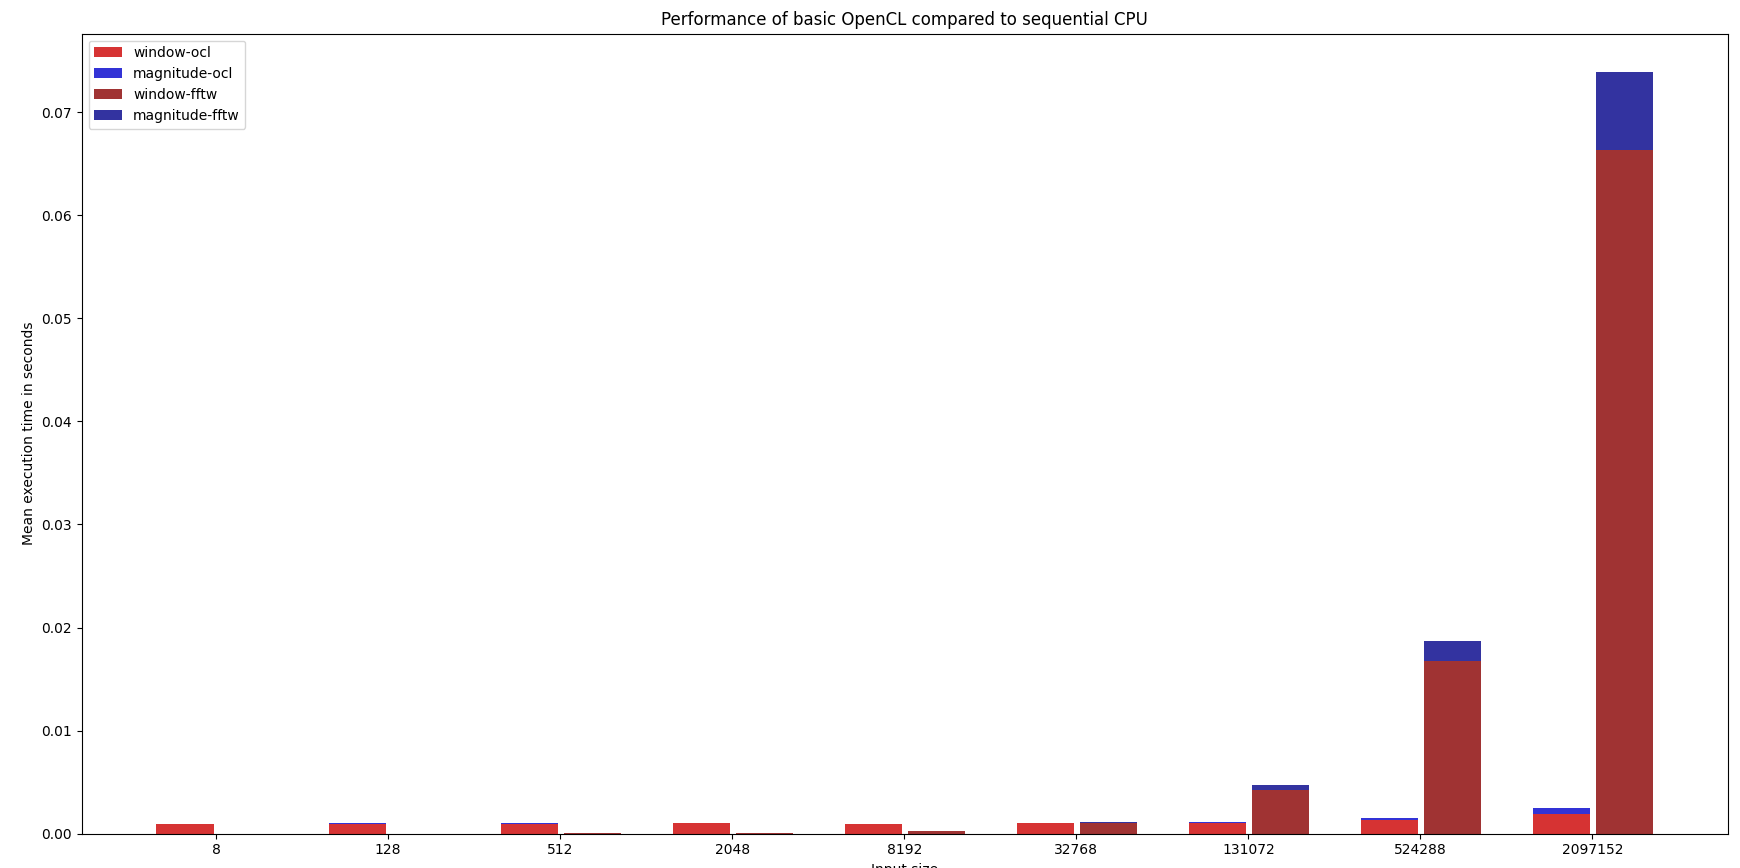
\includegraphics[width=0.9\textwidth]{resources/images/win-mag-ocl.png}
		\caption{Windowing + magnitude performance up to $2^{21}$ elements \\
		(host-device + device-host transfer time exceeds 16.66 ms at $2^{21}$)}
	\end{figure}
	\endgroup
\end{frame}

% \begin{frame}{}
% 	\begingroup
% 	\small
% 	\begin{figure}
% 		\centering
% 		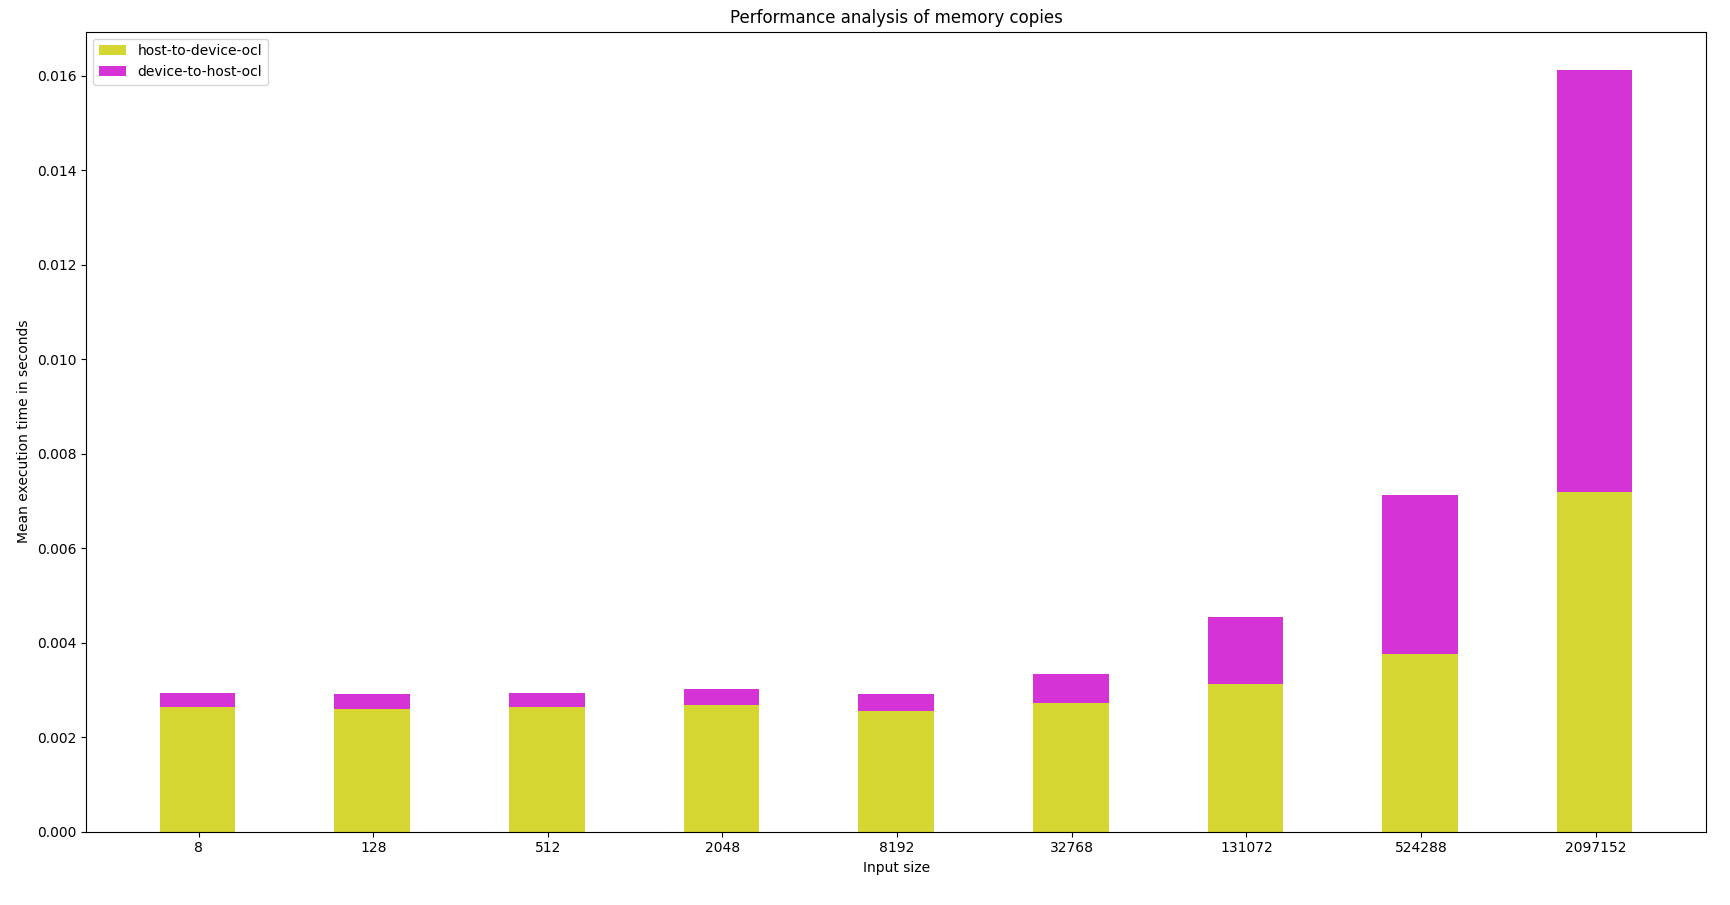
\includegraphics[width=1\textwidth]{resources/images/copies-ocl.png}
% 	\end{figure}
% 	\endgroup
% \end{frame}

\begin{frame}{}
	\begingroup
	\small
	\begin{figure}
		\cexternal{resources/c/seq-fft.c}
	\end{figure}
	\endgroup
\end{frame}

\begin{frame}{}
	\begingroup
	\small
	\begin{columns}
		\begin{column}{0.50\textwidth}
			Steps to achieve OpenCL FFT implementation
			\begin{itemize}
				\item On host lookup tables for\cinline{c1},\cinline{c2}
					,\cinline{l1} and\cinline{l2}
				\item \cinline{l1} and\cinline{l2} use same lookup table containing powers of two
				\item All three tables only contain one element per power of two
				\item Queue kernel per power of two
				\item Kernel range depends on current and past power of two
				\item Range emulates second and third loop levels from sequential
				\item \cinline{u1} and\cinline{u2} generated as OpenCL code
					using separate program
			\end{itemize}
		\end{column}
		\begin{column}{0.50\textwidth}
			\begin{figure}
				\csmallexternal{resources/c/schedule-fft.c}
			\end{figure}
		\end{column}
	\end{columns}
	\endgroup
\end{frame}

\begin{frame}{}
	\begingroup
	\small
	\begin{columns}
		\begin{column}{0.50\textwidth}
			\begin{figure}
				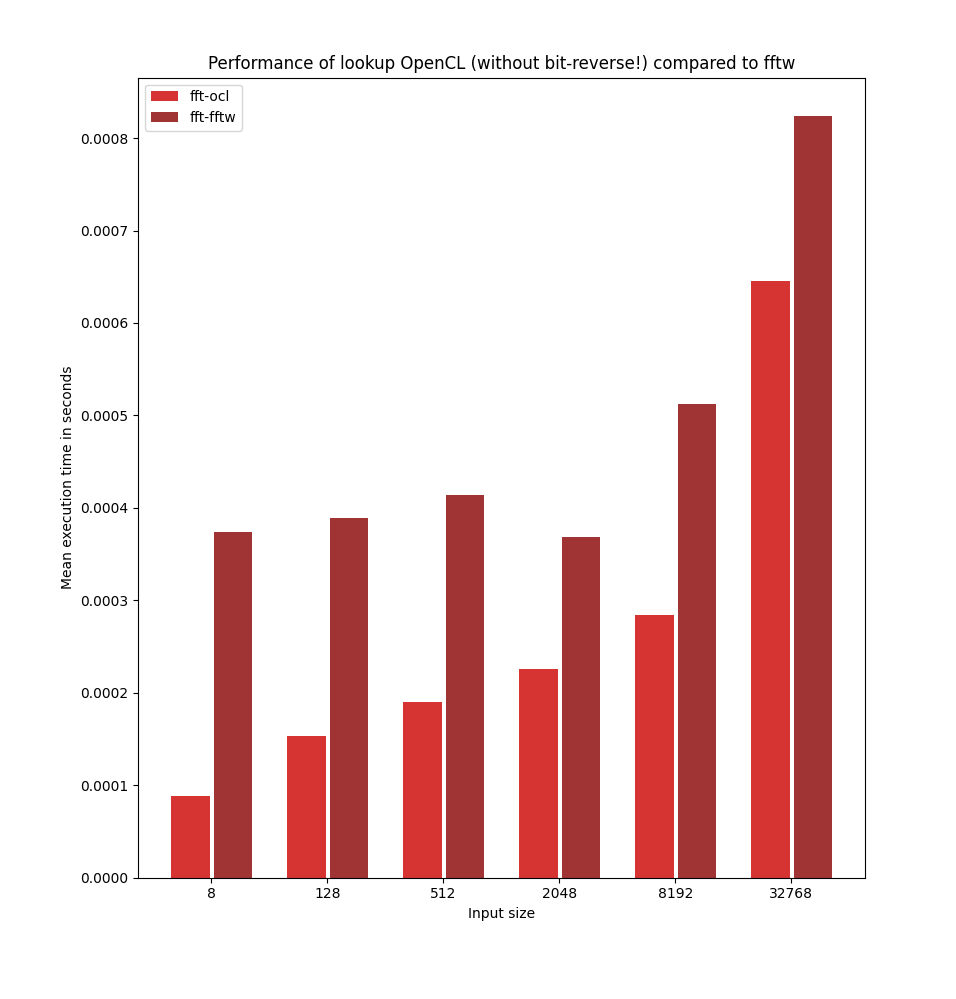
\includegraphics[width=1\textwidth]{resources/images/lookup-fft-low.png}
			\end{figure}
		\end{column}
		\begin{column}{0.50\textwidth}
			\begin{figure}
				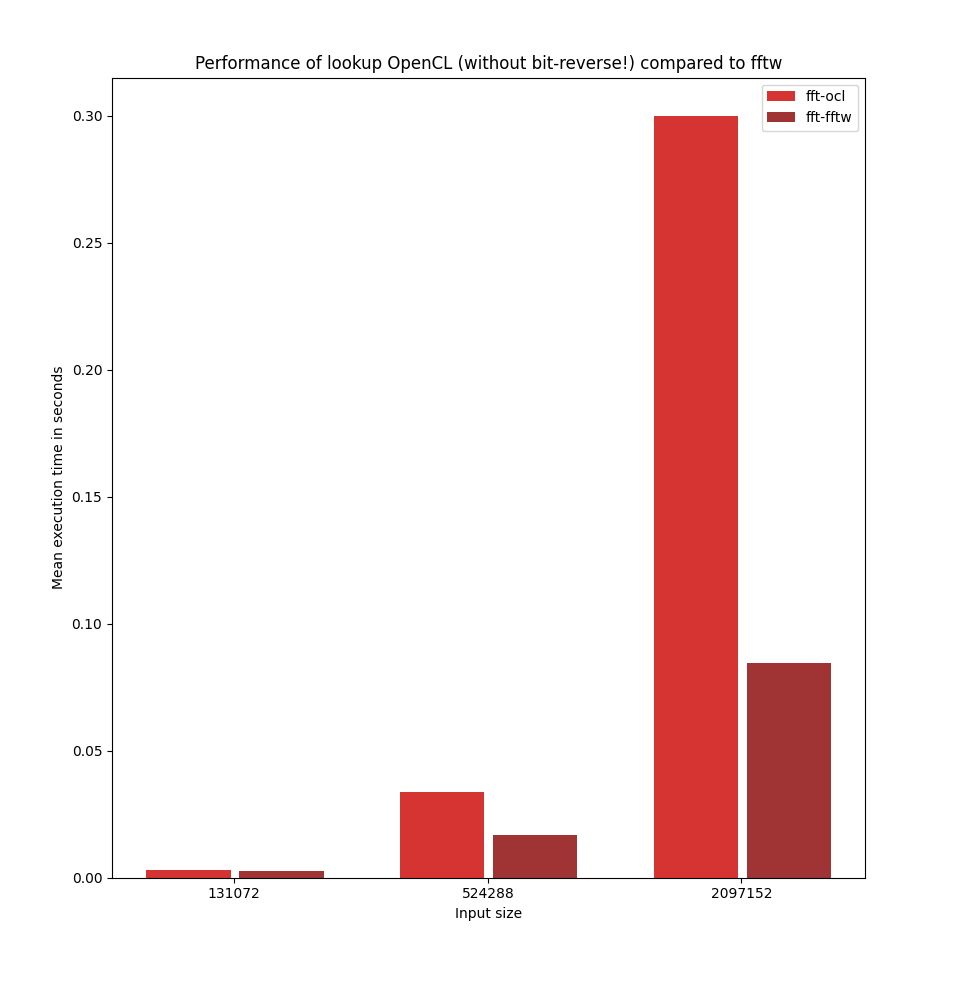
\includegraphics[width=1\textwidth]{resources/images/lookup-fft-high.png}
			\end{figure}
		\end{column}
	\end{columns}
	\endgroup
\end{frame}

\begin{frame}{}
	\begingroup
	\small
	OpenCL bit-reverse based on 2D array (matrix) manipulations
	\begin{columns}
		\begin{column}{0.50\textwidth}
				\begin{itemize}
					\item 1. Take index of columns as bit patterns up to $\log_2(N)/2$ bits
					\item 2. Create bit-reverse for each column index and put into lookup table
					\item 3. Swap every column with its bit-reverse for every row
					\item 4. Transpose the matrix
					\item 5. Repeat step 3
				\end{itemize}
		\end{column}
		\begin{column}{0.50\textwidth}
			\begin{figure}
				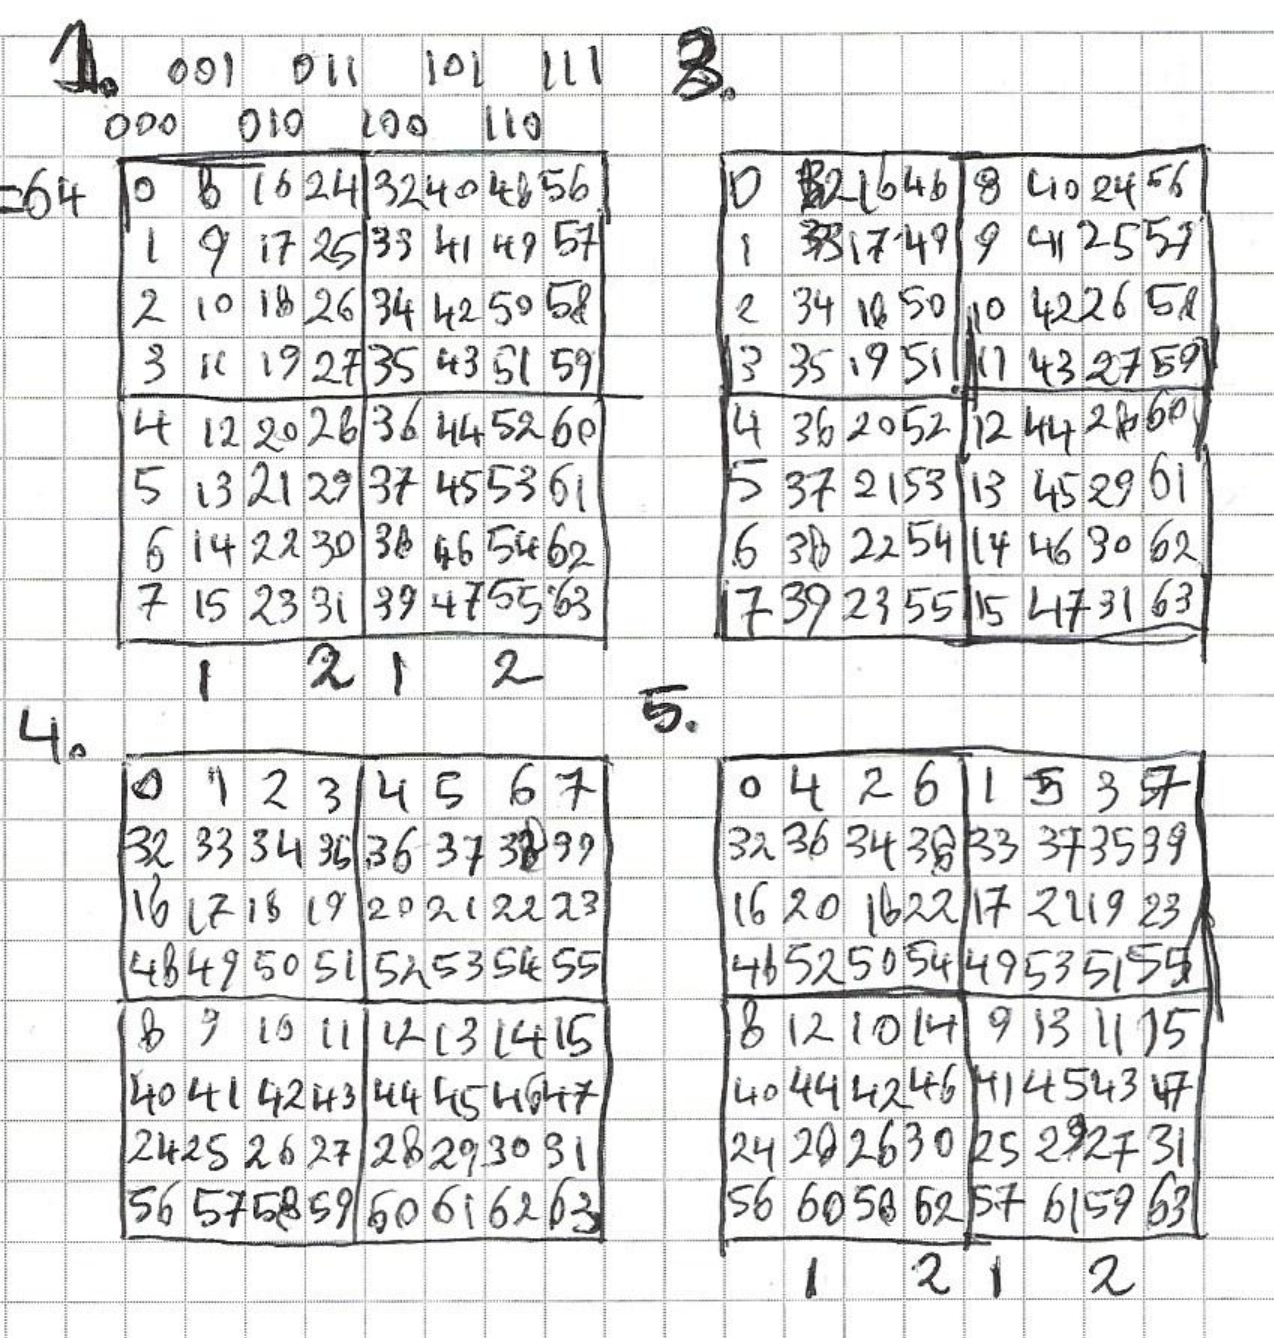
\includegraphics[width=0.8\textwidth]{resources/images/bit-reverse.png}
			\end{figure}
		\end{column}
	\end{columns}
	\endgroup
\end{frame}

\begin{frame}{}
	\begingroup
	\small
	\begin{columns}
		\begin{column}{0.50\textwidth}
			\begin{figure}
				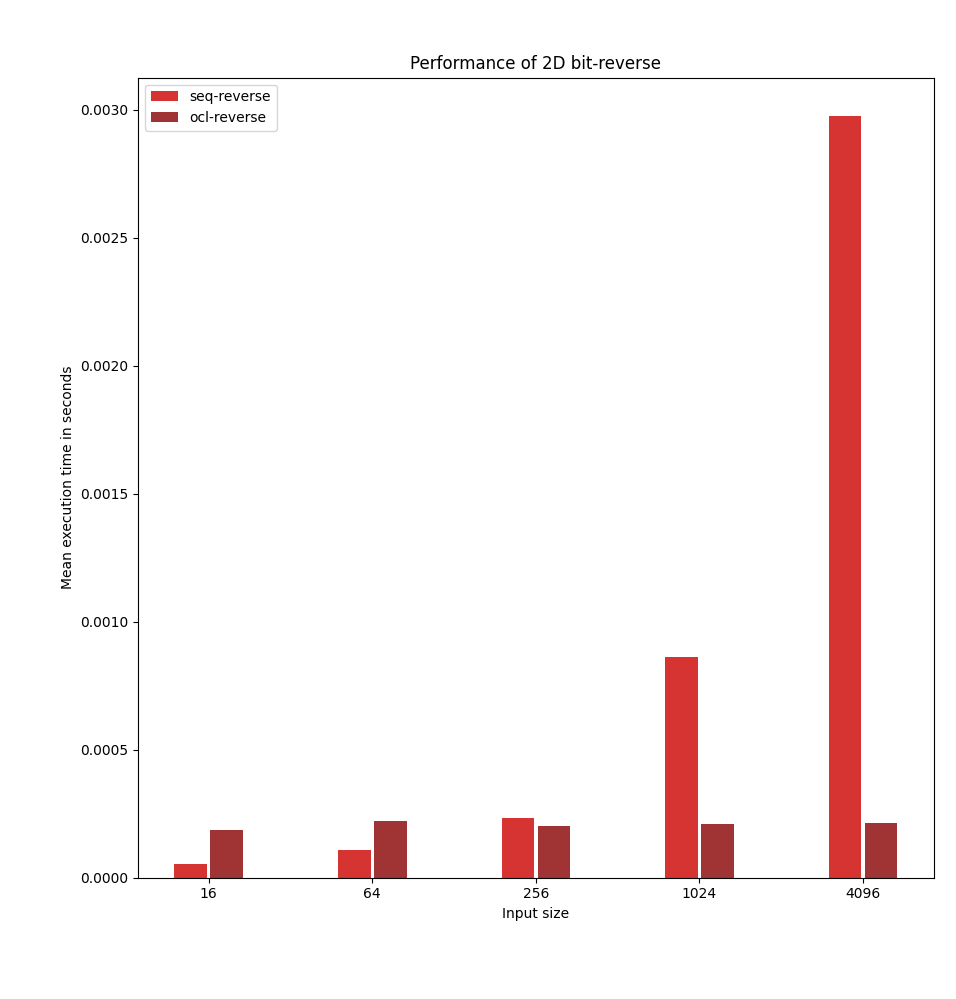
\includegraphics[width=1\textwidth]{resources/images/bit-reverse-low.png}
			\end{figure}
		\end{column}
		\begin{column}{0.50\textwidth}
			\begin{figure}
				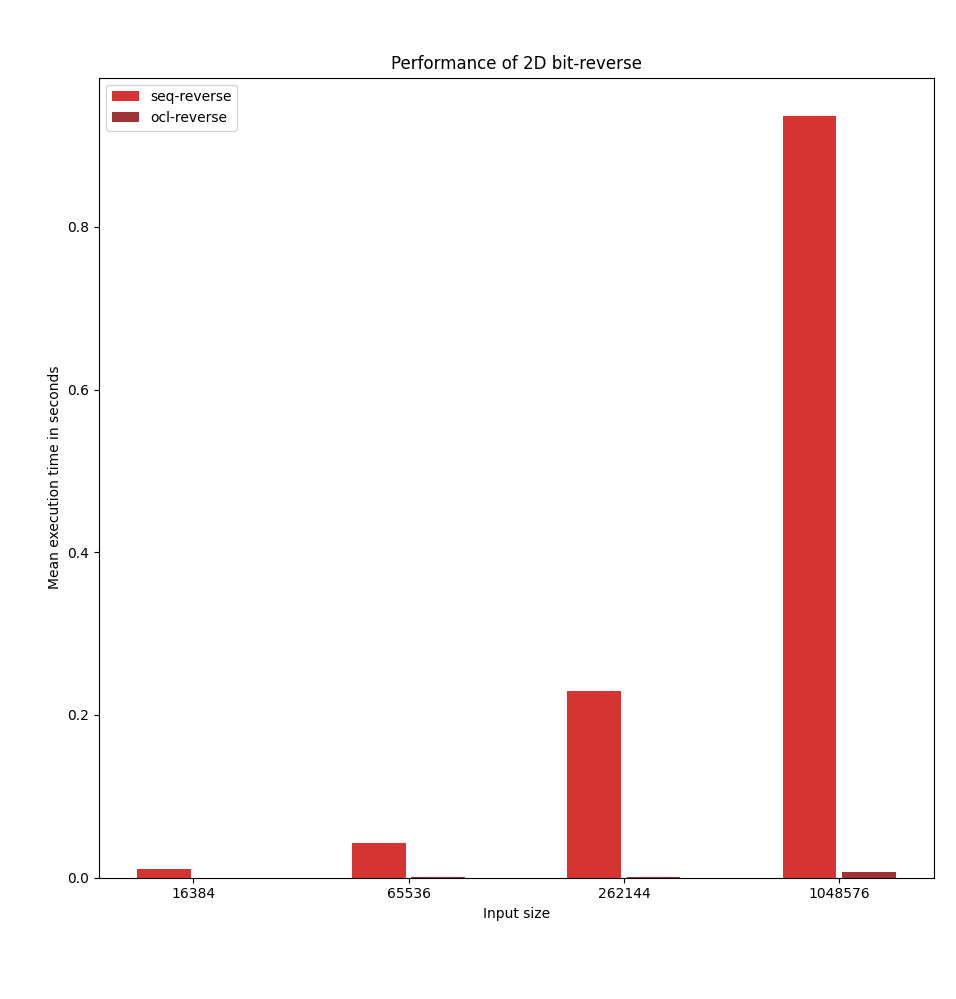
\includegraphics[width=1\textwidth]{resources/images/bit-reverse-high.png}
			\end{figure}
		\end{column}
	\end{columns}
	\endgroup
\end{frame}

\begin{frame}{}
	\begingroup
	\small
	\begin{figure}
		\centering
		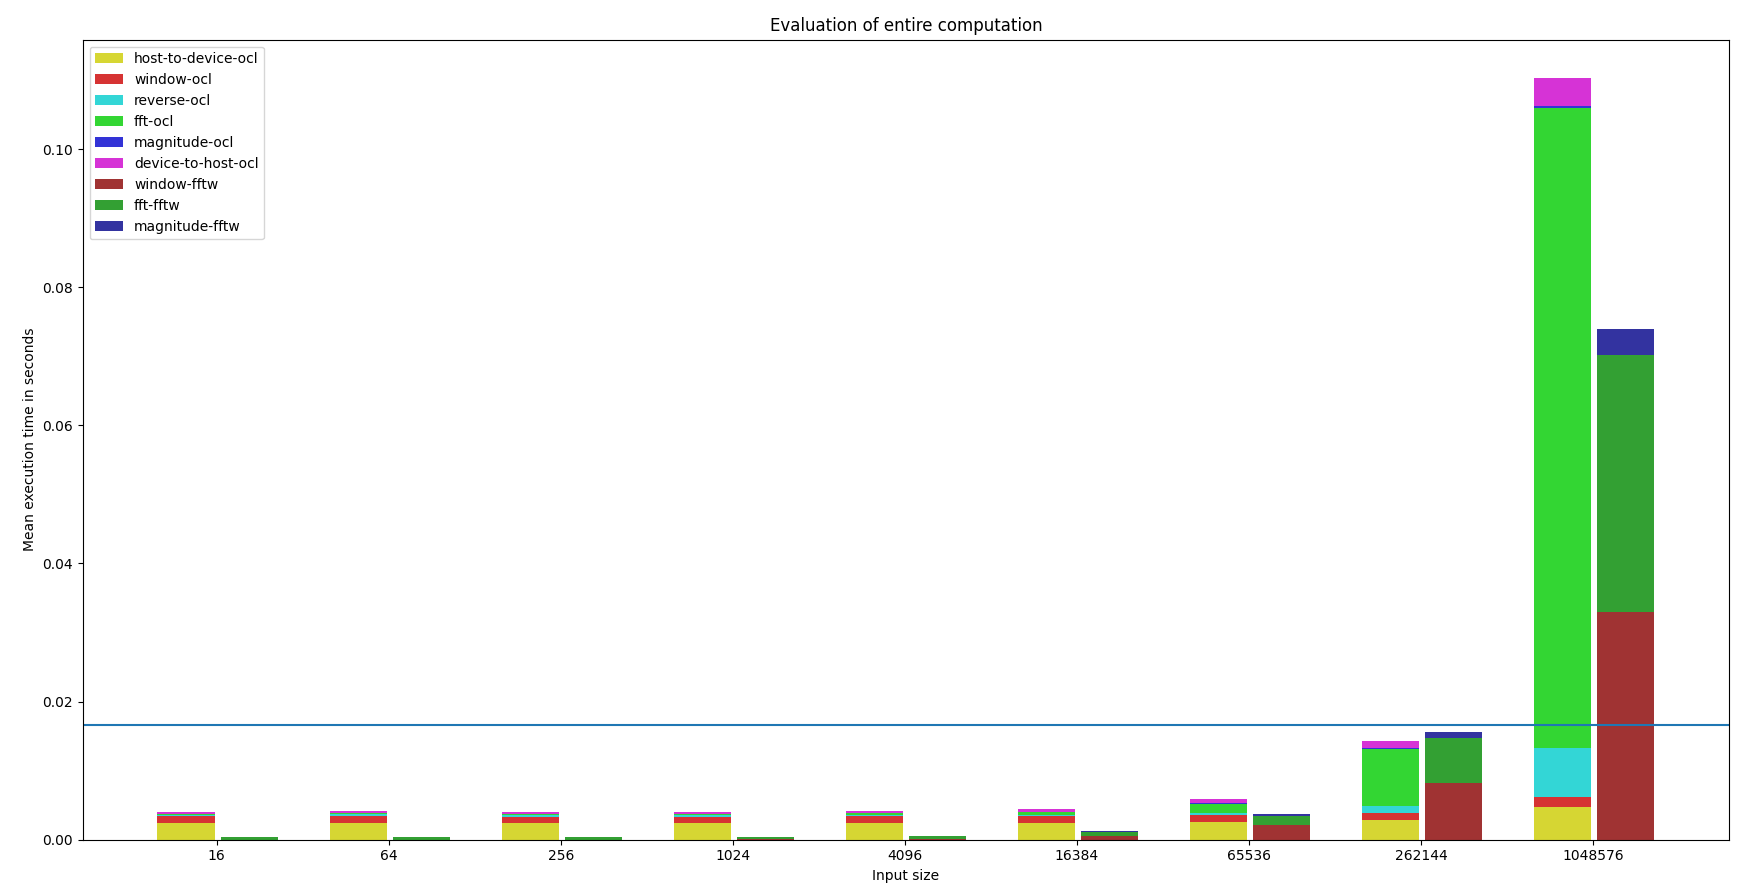
\includegraphics[width=0.9\textwidth]{resources/images/total-results.png}
	\end{figure}
	\endgroup
\end{frame}

\begin{frame}{Future work}
	\begingroup
	\small
	\begin{itemize}
		\item Condense OpenCL lookup as table for $2^{21}$ will contain
			entries of previous powers, offset formula non-trivial
		\item Evaluate Elster-Huff-Strandh recursive bit-reversal algorithm
			using nested parallelism
		\item Evaluate \textit{vanilla} Cooley-Tukey FFT using nested
			parallelism instead of bit-reverse
		\item Compare performance against cuFFT, rocFFT, clFFT and similar
	\end{itemize}
	\endgroup
\end{frame}

\end{document}